\section{Processi organizzativi}

\subsection{Gestione organizzativa}
\subsubsection{Scopo}
In questa sezione sono indicate le modalità di coordinamento del Team Oberon:
\begin{itemize}
    \item Adottare un modello organizzativo che consente di individuare anticipatamente i rischi;
    \item Specificare un modello di sviluppo da seguire;
    \item Rispettare le scadenze e le spese concordate; 
\end{itemize}
\subsubsection{Aspettative}
\begin{itemize}
    \item Assicurarsi una pianificazione ragionevole dei compiti da svolgere;
    \item Comunicazione chiara e priva di ambiguità tra i componenti del gruppo;
    \item Rientrare nei costi previsti regolando le attività;
    \item Distribuzione corretta ed equa dei ruoli di progetto;
\end{itemize}
\subsubsection{Descrizione}
\begin{itemize}
    \item Assegnazione dei ruoli e dei compiti;
    \item Inizio e definizione dello scopo;
    \item Istanziazione dei processi;
    \item Stima e pianificazione di costi, tempi e risorse;
    \item Esecuzione e controllo;
    \item Revisione e valutazione delle attività in modo periodico;
\end{itemize}
\subsubsection{Ruoli di progetto}
\subsubsection{Rapporti interpersonali tra i componenti del gruppo}
I componenti nel gruppo si impegnano a collaborare in modo pacifico e ben coordinato per facilitare la buona riuscita del progetto. \\
In particolare si cercherà il più possibile di lavorare in meeting a distanza per evitare errori o sviste e per motivare i vari membri. \\
I ruoli verranno assegnati ai componenti del gruppo in modo equo, affinché ogni persona possa svolgere tutti gli incarichi almeno una volta e per un numero di ore produttive adeguato. I ruoli di progetto vengono assegnati in concomitanza con l’inizio di un nuovo ciclo scrum per garantire coesione nel lavoro. \\
Tutte le comunicazioni riguardanti il progetto avverranno utilizzando il gruppo Telegram dedicato, queste possono includere:

\begin{itemize}
    \item pubblicazione/aggiornamento di un documento;
    \item richiesta di verifica di un documento;
    \item invito a collaborare su una particolare sezione del lavoro;
    \item confronto sulle disponibilità con i tempi per incontri con il proponente o i committenti;
    \item richiesta di feedback immediato su un particolare dubbio.
\end{itemize}


\subsection{Utilizzo delle infrastrutture interne}
\subsubsection{Gestione delle comunicazioni}
\subsubsection{Gestione degli incontri}
\subsubsection{Gestione degli strumenti di coordinamento}
\subsubsection{Gestione degli strumenti di versionamento}
\subsubsection{Gestione dei rischi}

\subsection{Formazione}

\subsection{Metodo di Sviluppo}
\subsubsection{Scrum}
Il Way of Working del team Oberon si basa sul framework Scrum, che prevede il raggiungimento dell’obiettivo finale del progetto tramite una serie di sprint, ognuno dei quali fissa un obiettivo intermedio da raggiungere e dura due settimane. 
\subsubsection{Eventi Sprint}
\begin{enumerate}
\item Sprint Planning, è la riunione che segna l’inizio dello sprint: il Team concorda l’obiettivo principale dello sprint e individua gli elementi del Product Backlog necessari al suo raggiungimento; 
\item Sprint Review, viene organizzata al termine di ogni sprint per valutare se l’obiettivo prefissato è stato raggiunto; 
\item Sprint Retrospective, è una riunione che serve al Team per identificare le cause di eventuali problemi che si sono verificati durante l’ultimo sprint e individuare dei miglioramenti da apportare al processo. 
\end{enumerate}
\subsubsection{Scaletta Scrum}
Durante ogni chiamata di fine scrum il team seguirà i seguenti passaggi:
\begin{enumerate}
    \item Aggiornamento dati sulla piattaforma Jira;
    \item Confronto tra obiettivi prefissati e raggiunti;
    \item Discussione delle problematiche riscontrate dai membri;
    \item Caricamento sulla repository dei file aggiornati;
    \item Definizione degli obiettivi dello scrum successivo;
    \item Assegnazione dei ruoli di ogni membro.
\end{enumerate}

\subsection{Tecnologie e Software}
\subsubsection{Elenco}
Il Team Oberon lavorerà in modalità asincrona utilizzando i seguenti software: Telegram, Discord e Google Meet, GitHub, Jira, StarUML, Microsoft Teams, Microsoft Project. \newline
\begin{center}
    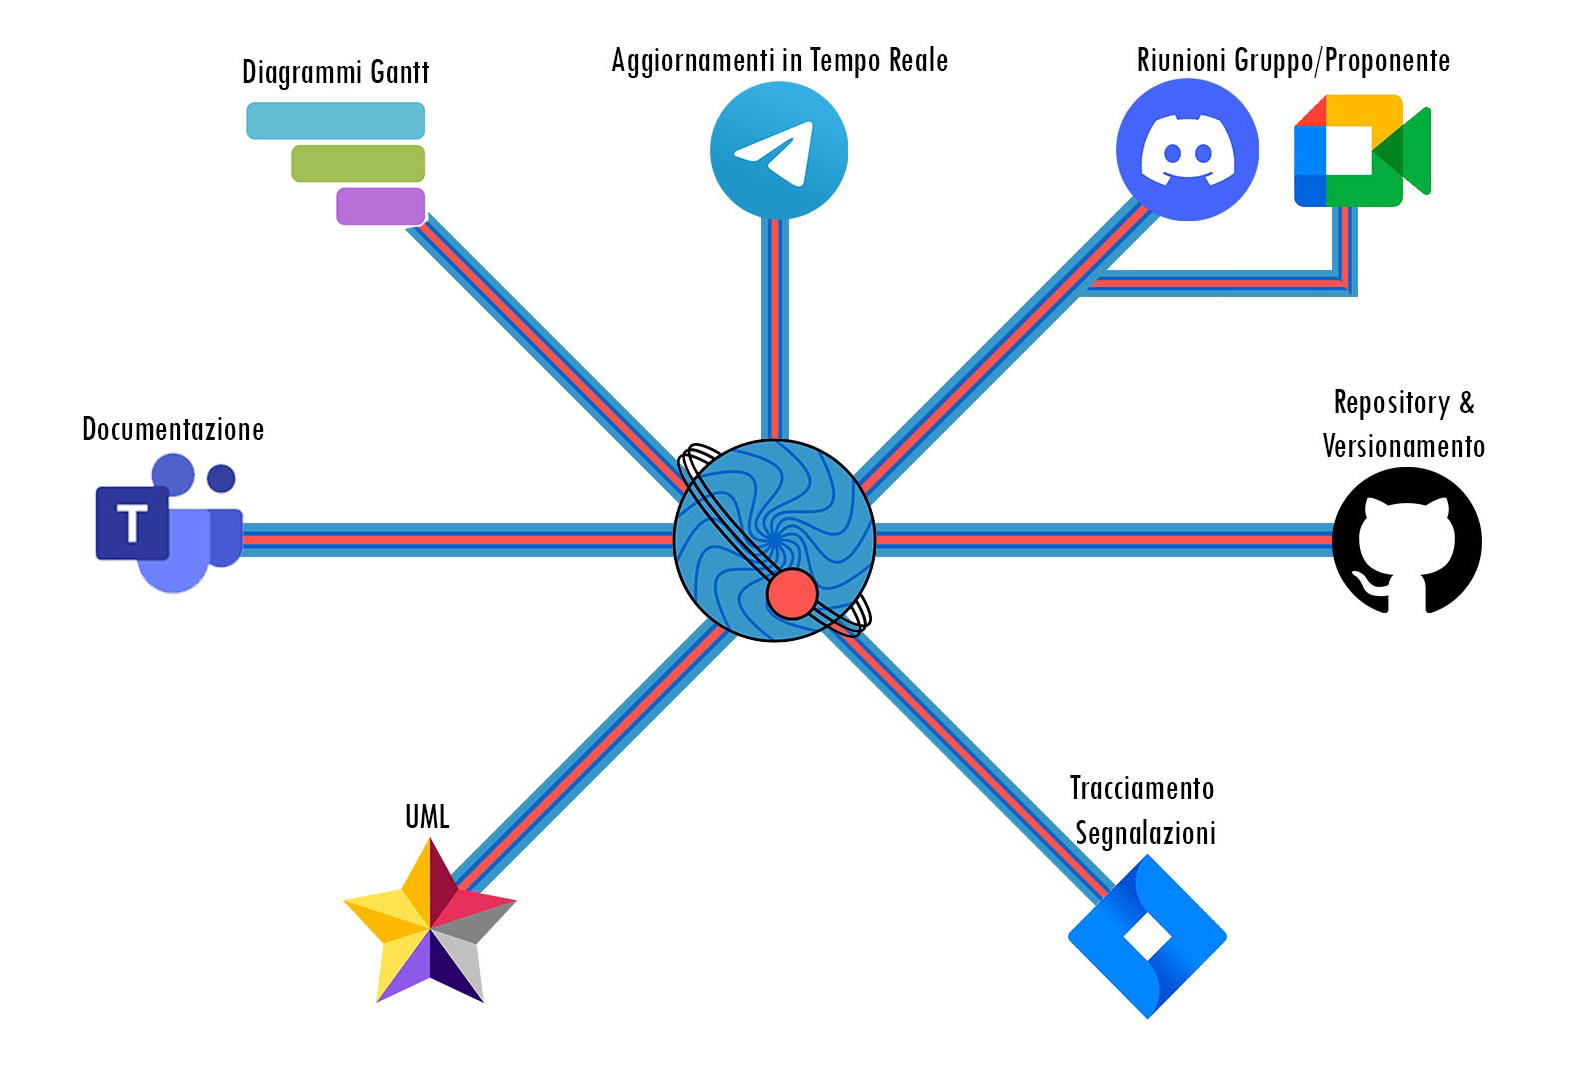
\includegraphics[scale = 1.0]{img/tecnologie.png}\\[1cm] 
\end{center}
Le tecnologie sono state scelte in accordo tra i singoli membri del gruppo, che si sono basati sulle proprie preferenze e conoscenze. In caso di problematiche nell’utilizzo di uno di questi software, il gruppo si riunirà per sostituirla. 
\subsubsection{Telegram}
La nota app di messagistica contiene un gruppo di cui ogni membro può usufruire per comunicare istantaneamente con tutti gli altri. Lo scopo principale consiste nel porre domande, chiarire dubbi e organizzare le riunioni. 
\subsubsection{Discord e Google Meet}
La prima di queste due piattaforme è stata consigliata dal proponente, il quale ha suggerito la creazione di un canale dedicato al gruppo, con il fine di facilitare la comunicazione con l’azienda stessa ed avere a disposizione un programma affidabile per eventuali meeting.  
\newline Il team ha usufruito di Google Meet durante le prime riunioni con l’azienda. 
\subsubsection{GitHub}
Il servizio hosting per progetti software GitHub è parso l’ideale per il versionamento del capitolato assegnato al team in quanto molto popolare per questi utilizzi. Inoltre il gruppo possiede una certa familiarità con esso. 
Ogni membro avrà una copia aggiornata del repository sulla quale lavorare. La regola principale imposta nell’utilizzo di GitHub consiste nell'effettuare commit solo nel caso di modifiche sostanziali ai file. 
\subsubsection{Jira}
Jira offre una funzionalità dashboard inclusa che raccoglie automaticamente i dati dalle issue create ed è particolarmente adatta al metodo di sviluppo di tipo scrum. Nel cruscotto del team Oberon si trovano: \newline
\noindent
\includegraphics[scale=0.55]{img/imgDashboard.PNG}

\paragraph{Ticketing}
Jira offre un sistema di ticketing con il quale è possibile assegnare i vari compiti legati al progetto ai membri. La maggior parte del tracking della dashboard è proprio legata alle issue create dal project manager del periodo e assegnate di comune accordo durante il meeting di chiusura scrum precedente.\\[0.1cm]
I ticket creati rappresentano singole attività da svolgere dal componente a cui sono state assegnate nel periodo di uno scrum specifico. Nel caso di due individui a cui è assegnata la stessa attività si applica una numerazione ordinata.\\[0.5cm]
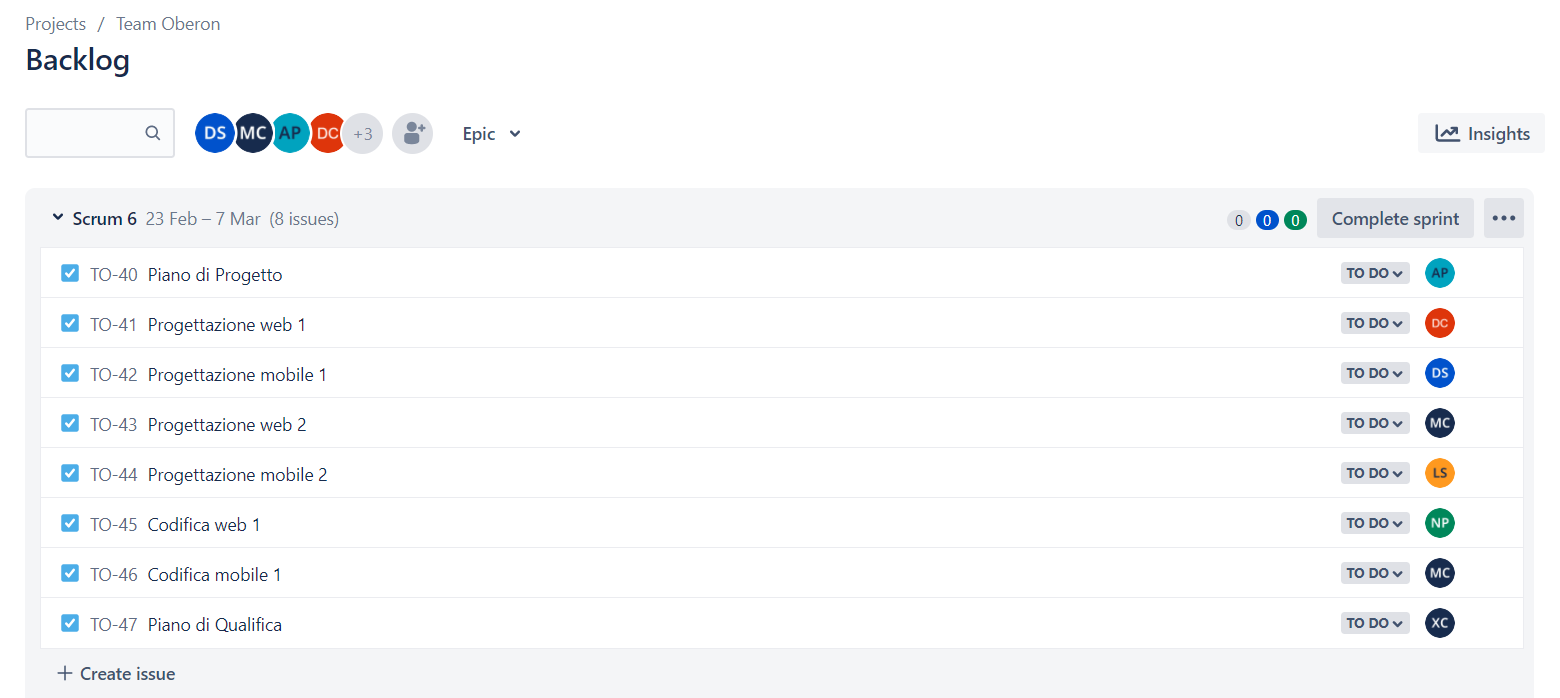
\includegraphics[scale=0.45]{img/issues.PNG}
\subsubsection*{Dashboard}
Jira offre una funzionalità dashboard inclusa che raccoglie automaticamente i dati dalle issue create ed è particolarmente adatta al metodo di sviluppo di tipo scrum.\\ Mantenere un'aggiornata rappresentazione grafica della distribuzione della mole di lavoro è fondamentale per tenere sotto controllo l'andamento del progetto e facilita la suddivisione dei compiti. \\[0.1cm]
Il project manager ha il compito di dedicare parte della sua attenzione alla dashboard per assicurare un buono svolgimento. \\[0.1cm]
Nel cruscotto del team Oberon si trovano: 
\newline
\noindent
\includegraphics[scale=0.55]{img/imgDashboard.PNG}

\subsubsection{TeamGantt}
Questo software è stato scelto per la produzione di diagrammi di gantt per la sua semplicità e per il fatto che è gratuito; è largamente sufficiente per gli scopi del gruppo.
\subsubsection{StarUML}
Gli schemi UML, diagrammi dei casi d'uso e di attività verranno prodotti con questo software.

\subsection{Ruoli di progetto}
\subsubsection{Rotazione dei ruoli}
Al termine di ogni scrum avverrà una rotazione dei ruoli. I ruoli disponibili sono Responsabile, Amministratore, Analista, Progettista, Programmatore e Verificatore.
\\\\
Ciascun componente del team dovrà:
\begin{itemize}
\setlength\itemsep{0.1em}
    \item assicurarsi di svolgere equamente ciascun ruolo (ogni ruolo almeno una volta, e non persistere sugli stessi ruoli);
    \item lavorare un numero di ore equo a quello degli altri componenti del team;
    \item mantenere una certa flessibilità, ossia in caso di necessità svolgere altri ruoli per aiutare i componenti del team in difficoltà.
\end{itemize}

\subsection{Gestione e codifica dei rischi}
I rischi di progetto vanno individuati dal responsabile, che dovrà renderli noti e descriverli all'interno del piano di progetto. Occorrerà inoltre monitorare i rischi già individuati, e ridefinire eventualmente le strategie di gestione.
\\\\
Per quanto riguarda la codifica, il formato del rischio è il seguente:
\begin{center}
    [Sigla][Numero]: Nome rischio
\end{center}
e le sigle possibili sono UM (rischio di natura umana) o TE (rischio di natura tecnologica).